\documentclass[14pt, aspectratio=169]{beamer}
\usepackage{Mystyle}
\usepackage{geometry}
\usepackage{graphicx}
\usepackage{amssymb}
\usepackage{amsmath}
\usepackage{amsthm}
\usepackage{empheq}
\usepackage{mdframed}
\usepackage{booktabs}
\usepackage{lipsum}
\usepackage{color}
\usepackage{psfrag}
\usepackage{tikz, pgfplots}   % For plotting beautiful graphs
\usepackage{bm}
\usepackage[english]{babel}
\usepackage{biblatex} 
\usepackage{csquotes} 
\usepackage{setspace}
\usepackage{multicol}  
\usepackage[skip=3pt plus 1pt, indent=30pt]{parskip}    % Setting space between paragraphs and indent
\usepackage[T1]{fontenc}    % Output font encoding for international characters
\usepackage{helvet}        % Selecting font family
\usepackage{ragged2e}      % For text alignment
\usepackage{adjustbox}       % For defining new environments
\usepackage{fancyhdr}       % For defining headers and footers
\usepackage[cochineal]{newtxmath}
\usepackage{caption}
\usetikzlibrary{positioning}
\usetikzlibrary{intersections}
\usetikzlibrary{decorations.text}
\usetikzlibrary{decorations.pathreplacing}

\usetheme{Copenhagen}
\usecolortheme{beaver}
\setbeamertemplate{navigation symbols}{}    % Remove navigation symbols
\setbeamertemplate{headline}{}  %Remove headlines
%\setbeamercovered{transparent}    % Transparent covered items


\title{Delay-locked loop}
\author{Luis Guillermo Macias Rojas}

\begin{document}
    \maketitle

    \begin{frame}
        \tableofcontents
    \end{frame}

    \section{Background}

    \begin{frame}{Where is it used?}
        \begin{itemize}
            \item<1-> The delay-locked loop (DLL) is a circuit that is used to align the phase of a clock signal with the phase of a reference signal.
            \item<2-> The DLL is used in applications where the phase of the clock signal is critical, such as in high-speed communication systems.
            \item<3-> Where you need a \alert<3>{PVT robust} clock distribution.
        \end{itemize}
    \end{frame}
    \section{Analysis}

    \subsection{Basic concepts}

    \begin{frame}{Skew in transmission lines}
        \begin{columns}
            \column{0.5\linewidth}
            \begin{itemize}
                \item<1-> Skew ($\Delta_T$) can be viewed as the difference in phase between two signals.
                \item<3-> If an interconnection's length is similar to that of the wave length ($\lambda$) of the signal, then a delay ($\Delta_{t_{TL}}$) will exist between A and B.
            \end{itemize}
            \vspace{0.4cm}
            \onslide<3->{\begin{equation*}
                \lambda = \frac{\nu_p}{f}
            \end{equation*}}
            \column{0.5\linewidth}
            \onslide<2->\begin{center}
                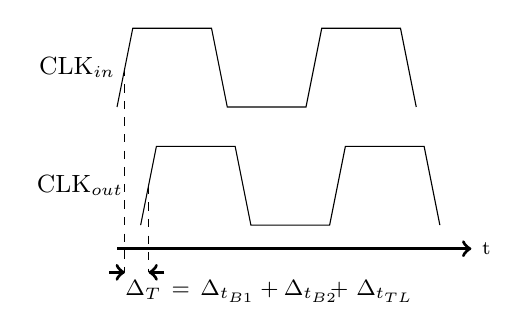
\begin{tikzpicture}
                    \draw (0,0) -- (0.2,1) -- (1.2,1) -- (1.4,0) -- (2.4,0) -- (2.6,1) -- (3.6,1) -- (3.8,0);   %CLK in
                    \draw (0.3,-1.5) -- (0.5,-0.5) -- (1.5,-0.5) -- (1.7,-1.5) -- (2.7,-1.5) -- (2.9,-0.5) -- (3.9,-0.5) -- (4.1,-1.5); %CLK out
                    \draw[dashed] (0.1,0.5) node[anchor=east]{\small{CLK$_{in}$}} -- (0.1,-2.1);  %dashed line
                    \draw[dashed] (0.4,-1) -- (0.4,-2.1);     %dashed line
                    \draw node[anchor=east] at (0.2,-1){\small{CLK$_{out}$}};
                    \draw[very thick, ->] (0,-1.8) -- (4.5,-1.8) node[anchor=west]{\scriptsize t};  %time arrow
                    \draw[->, very thick] (-0.1,-2.1) -- (0.1,-2.1);
                    \draw[->, very thick] (0.6,-2.1) -- (0.4,-2.1);
                    \draw node[anchor=north west, inner sep=0pt] at (0.1,-2.2) {\footnotesize $\Delta_T \, = \, \Delta_{t_{B1}} + \Delta_{t_{B2}}$};
                    \onslide<4->{\draw node[anchor=north west, inner sep=0pt] at (2.7,-2.2) {\footnotesize + \alert{$\Delta_{t_{TL}}$}};}
                \end{tikzpicture}
            \end{center}
            \vspace{0.5cm}
            \onslide<4->\begin{center}
                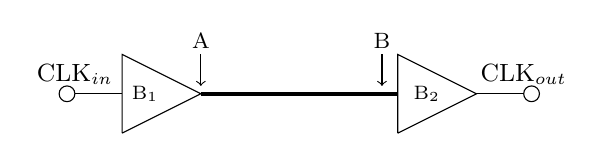
\begin{tikzpicture}
                    \draw (0,0) -- (0,1) -- (1,0.5) -- (0,0);   %buffer 1
                    \draw[ultra thick] (1, 0.5) -- (3.5,0.5);     %Transmission line
                    \draw (3.5,0) -- (3.5,1) -- (4.5,0.5) -- (3.5,0);   %buffer 2
                    \draw (-0.6,0.5) node[anchor=south]{\small CLK$_{in}$} -- (0,0.5) node[anchor=west]{\scriptsize B$_1$};
                    \draw (5.1,0.5) node[anchor=south]{\small CLK$_{out}$} -- (4.5,0.5) node[anchor=east, inner sep=13pt]{\scriptsize B$_2$};
                    \draw (-0.7,0.5) circle (0.1);  %terminal in
                    \draw (5.2,0.5) circle (0.1);   %terminal out
                    \draw[->] (1,1) node[anchor=south, inner sep=2pt]{\footnotesize A} -- (1,0.6);
                    \draw[->] (3.3,1) node[anchor=south, inner sep=2pt]{\footnotesize B} -- (3.3,0.6);
                \end{tikzpicture}
            \end{center}
        \end{columns}
    \end{frame}

    \begin{frame}{Skew correction}
        \begin{columns}
            \column{0.5\linewidth}
            \begin{itemize}
                \item<1-> How can we align CLK$_{out}$ with CLK$_{in}$ ?
                \item<2-> Since CLK$_{in}$ is periodic, an additional delay can be introduced at B$_2$ so as to make the total delay equal to once clock cycle (T$_{CLK}$).
            \end{itemize}
            \column{0.5\linewidth}
            \onslide<2->\begin{center}
                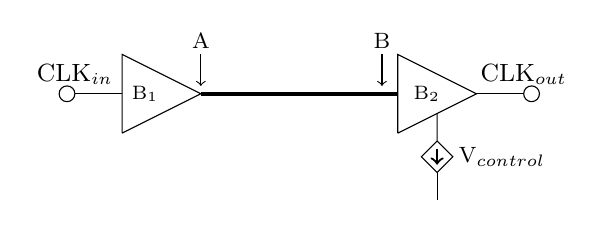
\begin{tikzpicture}
                    \draw (0,0) -- (0,1) -- (1,0.5) -- (0,0);   %buffer 1
                    \draw[ultra thick] (1, 0.5) -- (3.5,0.5);     %Transmission line
                    \draw (3.5,0) -- (3.5,1) -- (4.5,0.5) -- (3.5,0);   %buffer 2
                    \draw (4,0.25) -- (4,-0.1) -- (3.8,-0.3) --(4,-0.5) -- (4.2,-0.3) node[anchor=west, inner sep=2pt] {\footnotesize V$_{control}$} -- (4,-0.1);
                    \draw (4,-0.5) -- (4,-0.85);
                    \draw[->, thick] (4,-0.2) -- (4,-0.4);
                    \draw (-0.6,0.5) node[anchor=south]{\small CLK$_{in}$} -- (0,0.5) node[anchor=west]{\scriptsize B$_1$};
                    \draw (5.1,0.5) node[anchor=south]{\small CLK$_{out}$} -- (4.5,0.5) node[anchor=east, inner sep=13pt]{\scriptsize B$_2$};
                    \draw (-0.7,0.5) circle (0.1);  %terminal in
                    \draw (5.2,0.5) circle (0.1);   %terminal out
                    \draw[->] (1,1) node[anchor=south, inner sep=2pt]{\footnotesize A} -- (1,0.6);
                    \draw[->] (3.3,1) node[anchor=south, inner sep=2pt]{\footnotesize B} -- (3.3,0.6);
                \end{tikzpicture}
            \end{center}
            \vspace{0.5cm}
            \onslide<3->\begin{center}
                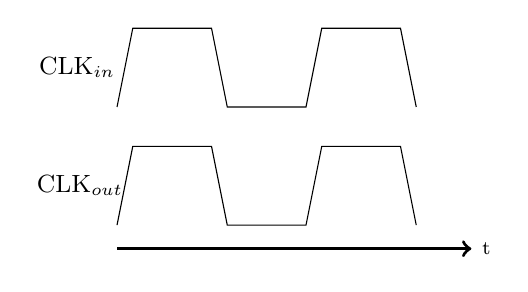
\begin{tikzpicture}
                    \draw (0,0) -- (0.2,1) -- (1.2,1) -- (1.4,0) -- (2.4,0) -- (2.6,1) -- (3.6,1) -- (3.8,0);   %CLK in
                    \draw (0,-1.5) -- (0.2,-0.5) -- (1.2,-0.5) -- (1.4,-1.5) -- (2.4,-1.5) -- (2.6,-0.5) -- (3.6,-0.5) -- (3.8,-1.5); %CLK out
                    \draw node[anchor=east] at (0.1,0.5) {\small CLK$_{in}$};
                    \draw node[anchor=east] at (0.2,-1) {\small CLK$_{out}$};
                    \draw[very thick, ->] (0,-1.8) -- (4.5,-1.8) node[anchor=west]{\scriptsize t};  %time arrow
                \end{tikzpicture}
            \end{center}
        \end{columns}
    \end{frame}

    \begin{frame}{DLL as a black box}
        
        \begin{columns}
            \column{0.5\linewidth}
            \begin{itemize}
                \item<1-> The DLL can be modeled as a box that takes in a control voltage and CLK$_{in}$, and outputs CLK$_{out}$ in phase with the reference.
            \end{itemize}
            \column{0.5\linewidth}
            \onslide<2->\begin{center}
                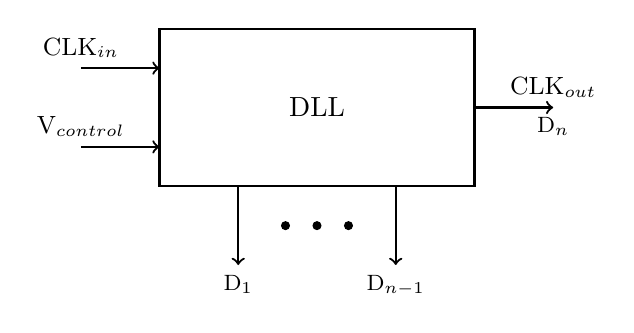
\begin{tikzpicture}
                    \draw[thick] (0,0) rectangle (4,2);
                    \draw node at (2,1) {DLL};
                    \draw[->, thick] (-1,1.5) node[anchor=south] {\small CLK$_{in}$} -- (0,1.5);
                    \draw[->, thick] (-1,0.5) node[anchor=south] {\small V$_{control}$} -- (0,0.5);
                    \draw[->, thick] (4,1) -- (5,1) node[anchor=south] {\small CLK$_{out}$};
                    \onslide<4->{\draw node[anchor=north] at (5,1) {\footnotesize D$_n$};}
                    \onslide<4->{\draw[->, thick] (1,0) -- (1,-1) node[anchor=north] {\footnotesize D$_1$};}
                    \onslide<4->{\filldraw (1.6,-0.5) circle (0.05);}
                    \onslide<4->{\filldraw (2,-0.5) circle (0.05);}
                    \onslide<4->{\filldraw (2.4,-0.5) circle (0.05);}
                    \onslide<4->{\draw[->, thick] (3,0) -- (3,-1) node[anchor=north] {\footnotesize D$_{n-1}$};}
                \end{tikzpicture}
            \end{center}
        \end{columns}
        \vspace{1cm}
        \begin{block}{Why use a DLL at all?}<3->
            \onslide<4->Because of $\Delta_{t_{TL}}$ and the DLL's ability to generate multiple phases.
        \end{block}
    \end{frame}
    \section{Design}

    \begin{frame}{Design of the DLL}
        \begin{itemize}
            \item<1-> The DLL is composed of a phase detector, a charge pump, a loop filter, and a voltage-controlled delay line.
            \item<2-> The phase detector compares the phase of the reference signal with the phase of the feedback signal and generates an error signal.
            \item<3> The charge pump convert of the voltage-controlled delay line.
        \end{itemize}

        \begin{example}<3>
            This is a cp deign example.
        \end{example}

    \end{frame}

    \begin{frame}{two column design}
        \begin{columns}
            \column{0.5\textwidth}
            lkadjhv;kaj;vkja;vn;;;;ncolum1 column1 akj;akj;av;asadbadbaab
            \column{0.5\textwidth}
            column2 a;fwkjap;hvah;v;ahav;av'a;jv;lajvlajvlkv'lkas'v;ksa'vk'svasvav
        \end{columns}
    \end{frame}

\end{document}